%%%%%%
%$Autor: Wings$
%$Projekt: A25-12$
%$Dateiname: ArduinoIDE2Mac.tex$
%$Beschreibung: Installation und Überblick zu Funktionen und Tools der Arduino IDE fir OS Geräte$
%%%%%%


\section{Installation der Arduino IDE für MacOS}

Der Download der Arduino IDE erfolgt über die Website \HREF{Arduino.cc}. Geben Sie dazu 
\glqq Arduino IDE Download \grqq in Ihren Browser ein. Nach Öffnen des ersten Sucheintrages kann nun die zum Betriebssystem passende Version der Arduino IDE im Auswahlfenster gewählt und mittels Doppelklick des Download Buttons heruntergeladen werden (vgl. \ref{pic:IDEMac01}). 

\begin{center}
	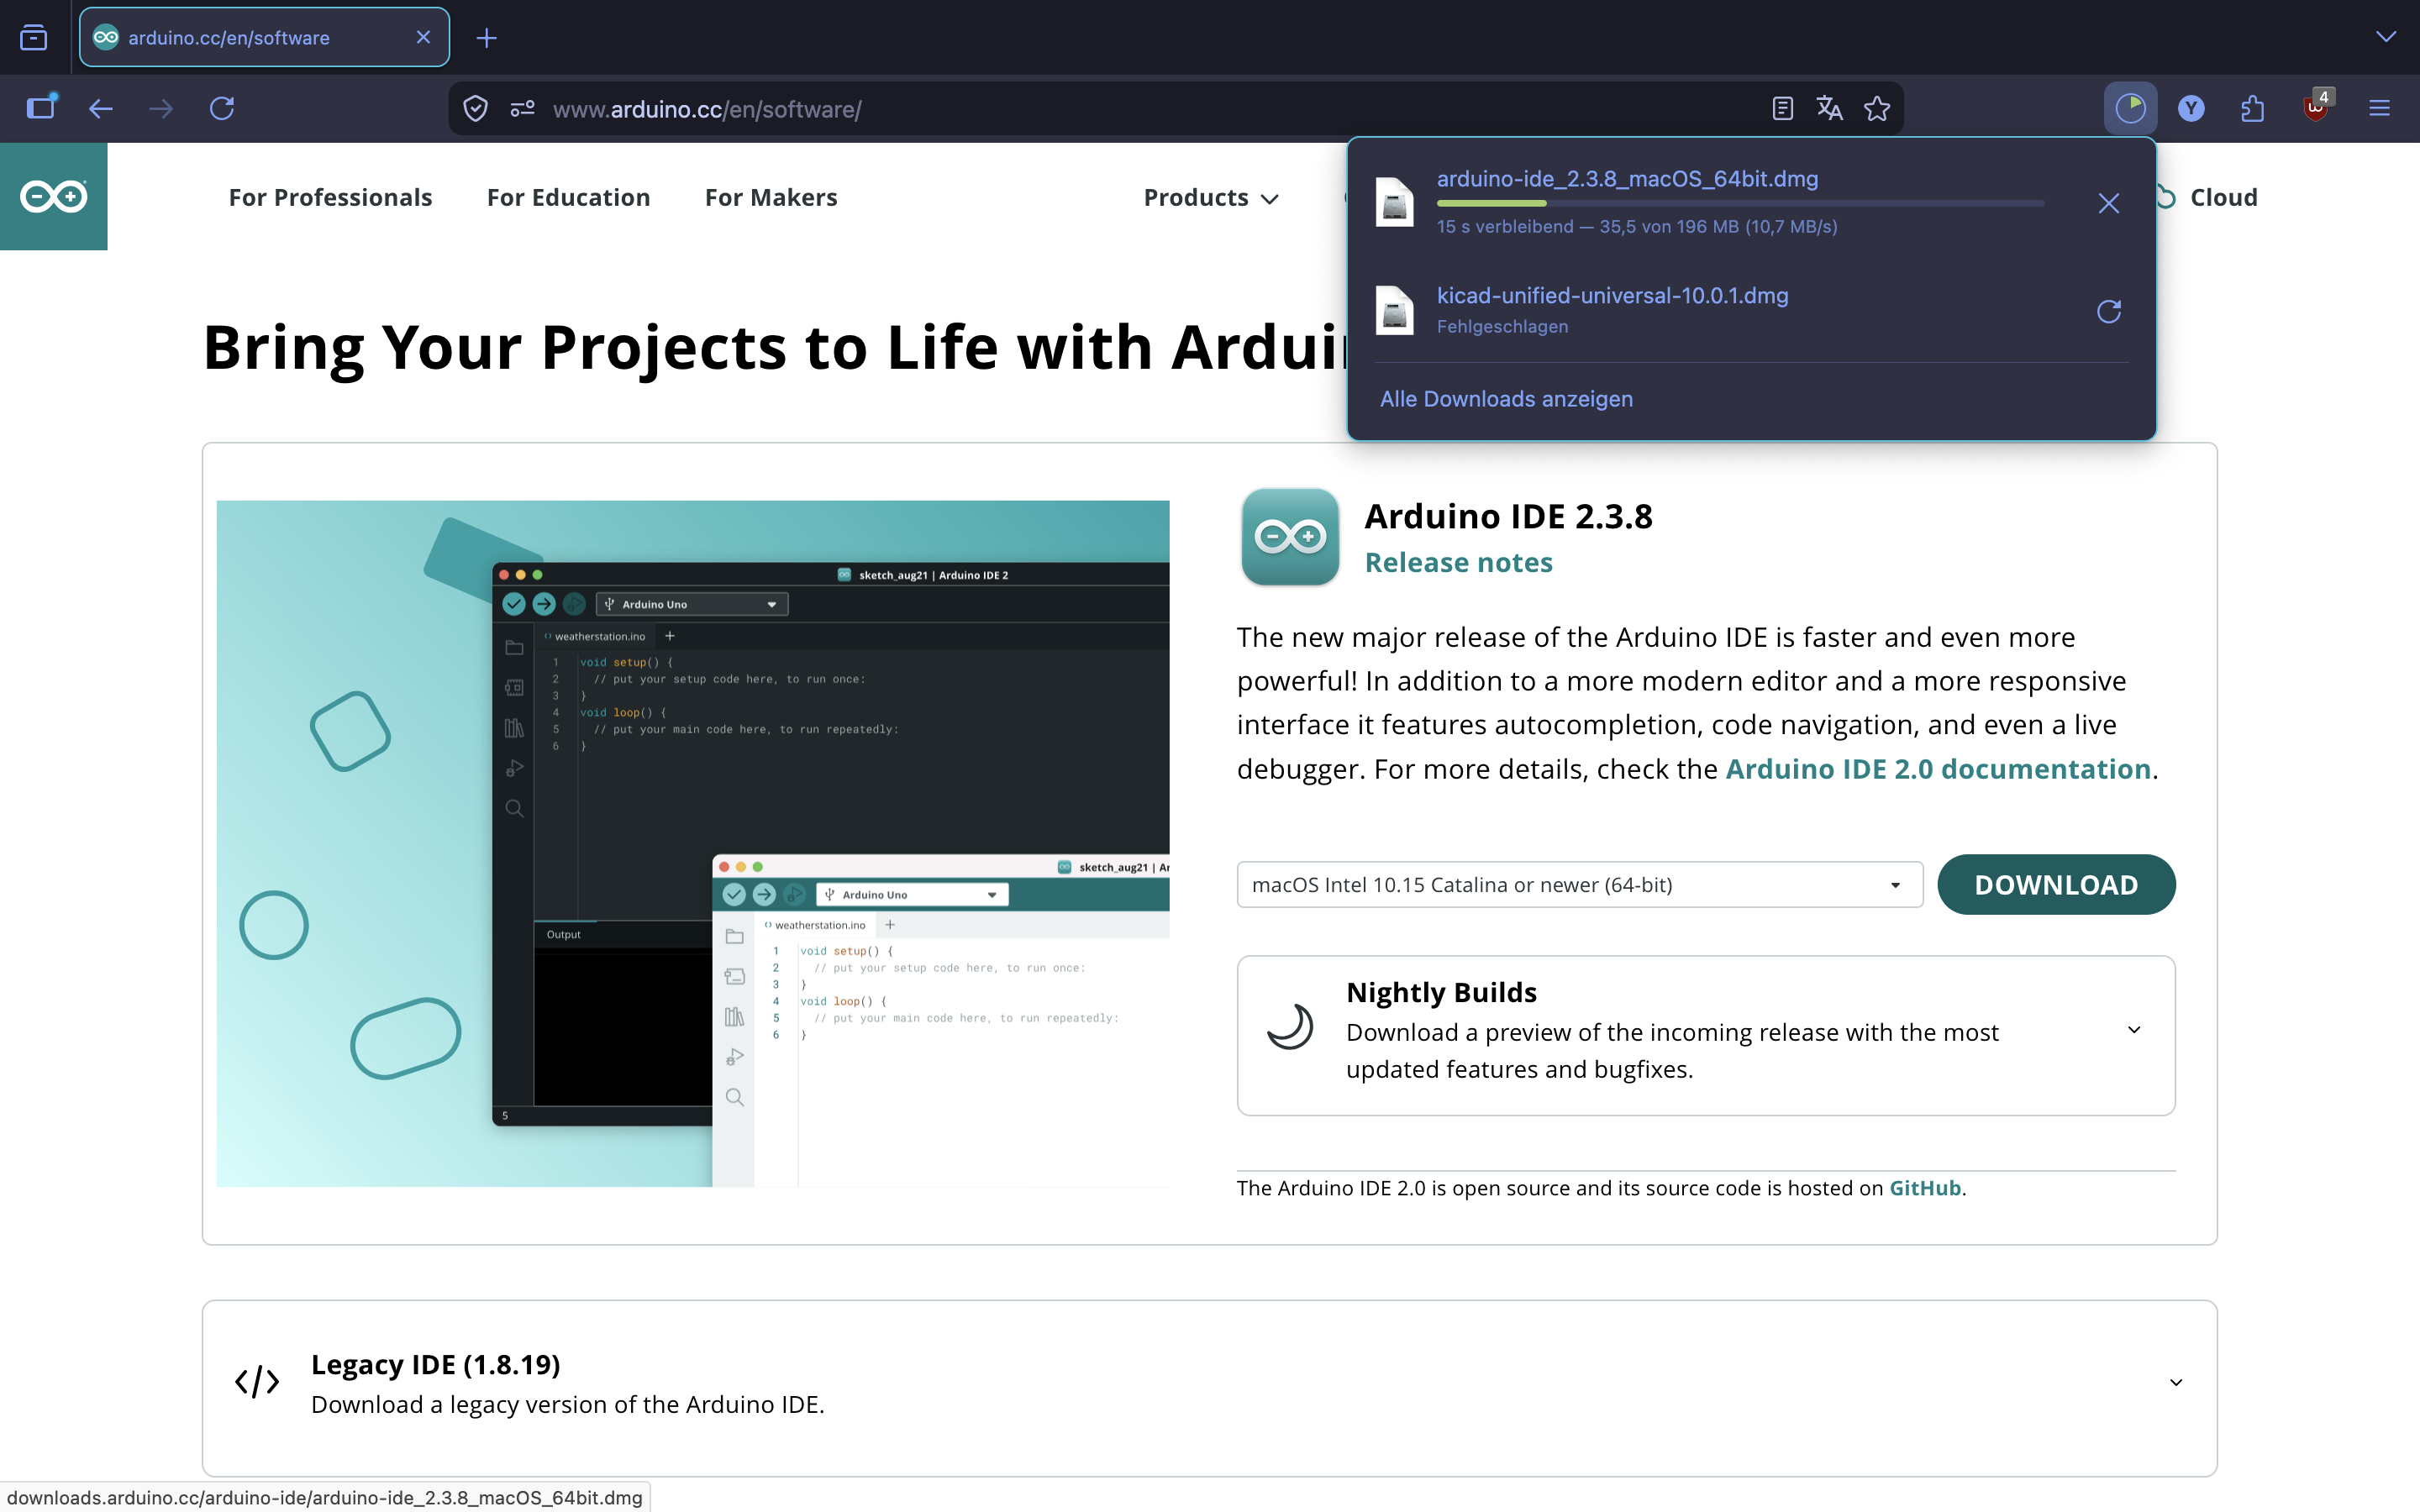
\includegraphics[width=1\textwidth,keepaspectratio]{../../Images/ArduinoIDE/MacOS/downloadfenster}
	\captionof{figure}{Aufruf der Arduino-Download-Webseite über die Suchmaschine}
	\label{pic:IDEMac01}
\end{center}

Der Download einer Datei im DMG Format wird standardmäßig im  \textcolor{blue}{Download Ordner} des Apple Dateimamnagmentsystems \textcolor{blue}{Finder} 
Dort kann die Datei dann mittels Doppelklick geöffnet werden (vgl. \ref{pic:FinderDownload} )

\begin{center}
	\begin{figure}
		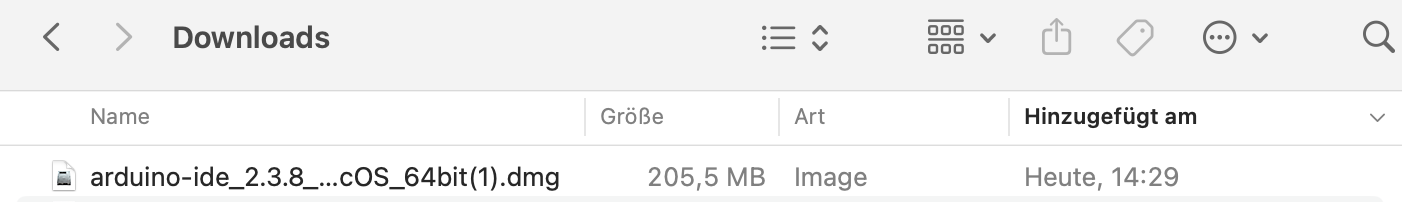
\includegraphics[width=1\textwidth,keepaspectratio]{../../Images/ArduinoIDE/MacOS/DownloadFinder}
		\caption{Heruntergeladene Installationsdatei der Arduino IDE im MacOS Finder. }
		\label{pic:FinderDownload}
	\end{figure}
\end{center}

Wie auf dem Betriebssystem MacOs üblich, muss jetzt lediglich die Installationsdatei in den Programmordner verschoben werden, und schon lässt sich die Arduino IDE als Programm öffnen (vgl. \ref{pic:ProgrammOrdner}). 

\begin{center}
	\begin{figure}
		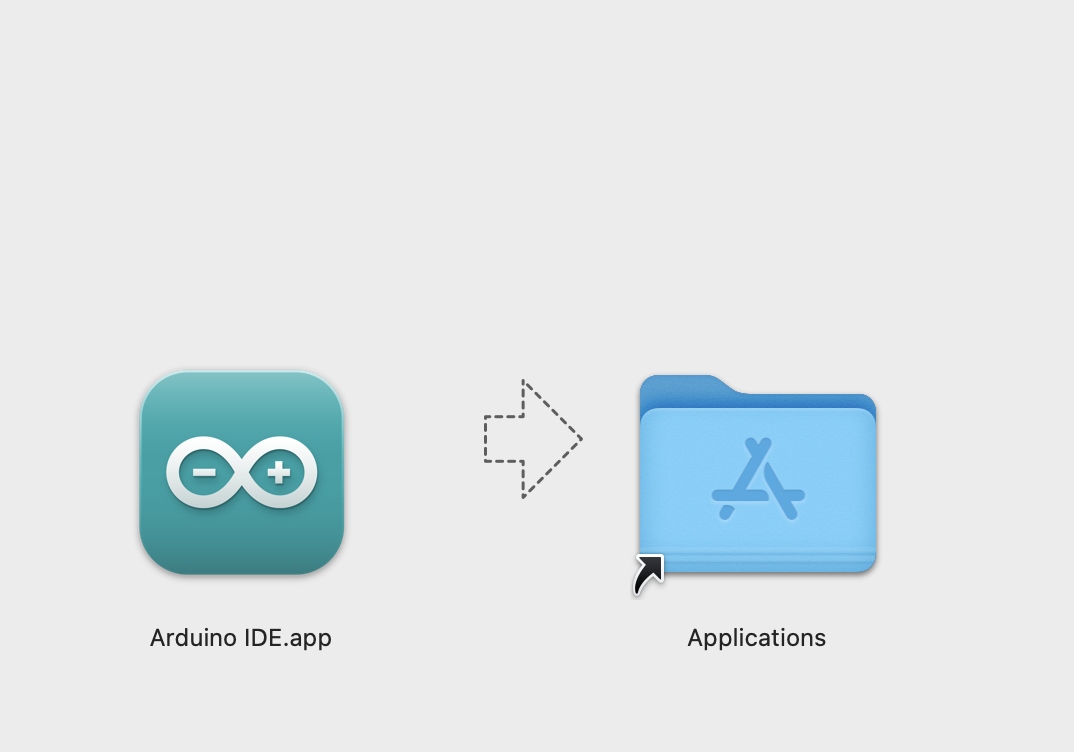
\includegraphics[width=1\textwidth,keepaspectratio]{../../Images/ArduinoIDE/MacOS/InProgrammordner}
		\caption{Fenster nach Öffnen der Installationsdatei zum Verschieben in den Programmordner }
		\label{pic:ProgrammOrdner}
	\end{figure}
\end{center}
Anschließen kann die Arduino IDE als Programm ausgeführt werden. Nun öffnet sich standardmäßig die zuletzt benutzte Arduino Datei. Auch kann nun die Konfiguration der Arduino IDE und des Mikrokontrollers vorgenommen werden. 
So kann das verwendete Board ausgewählt oder in die bestehende Datenbank der Boards hinzugefügt werden. Auch können Bibliotheken hinzugefügt udn installiert werden (vgl. \ref{pic:ArduinoIDEGUIMac})

\begin{center}
\begin{figure}
	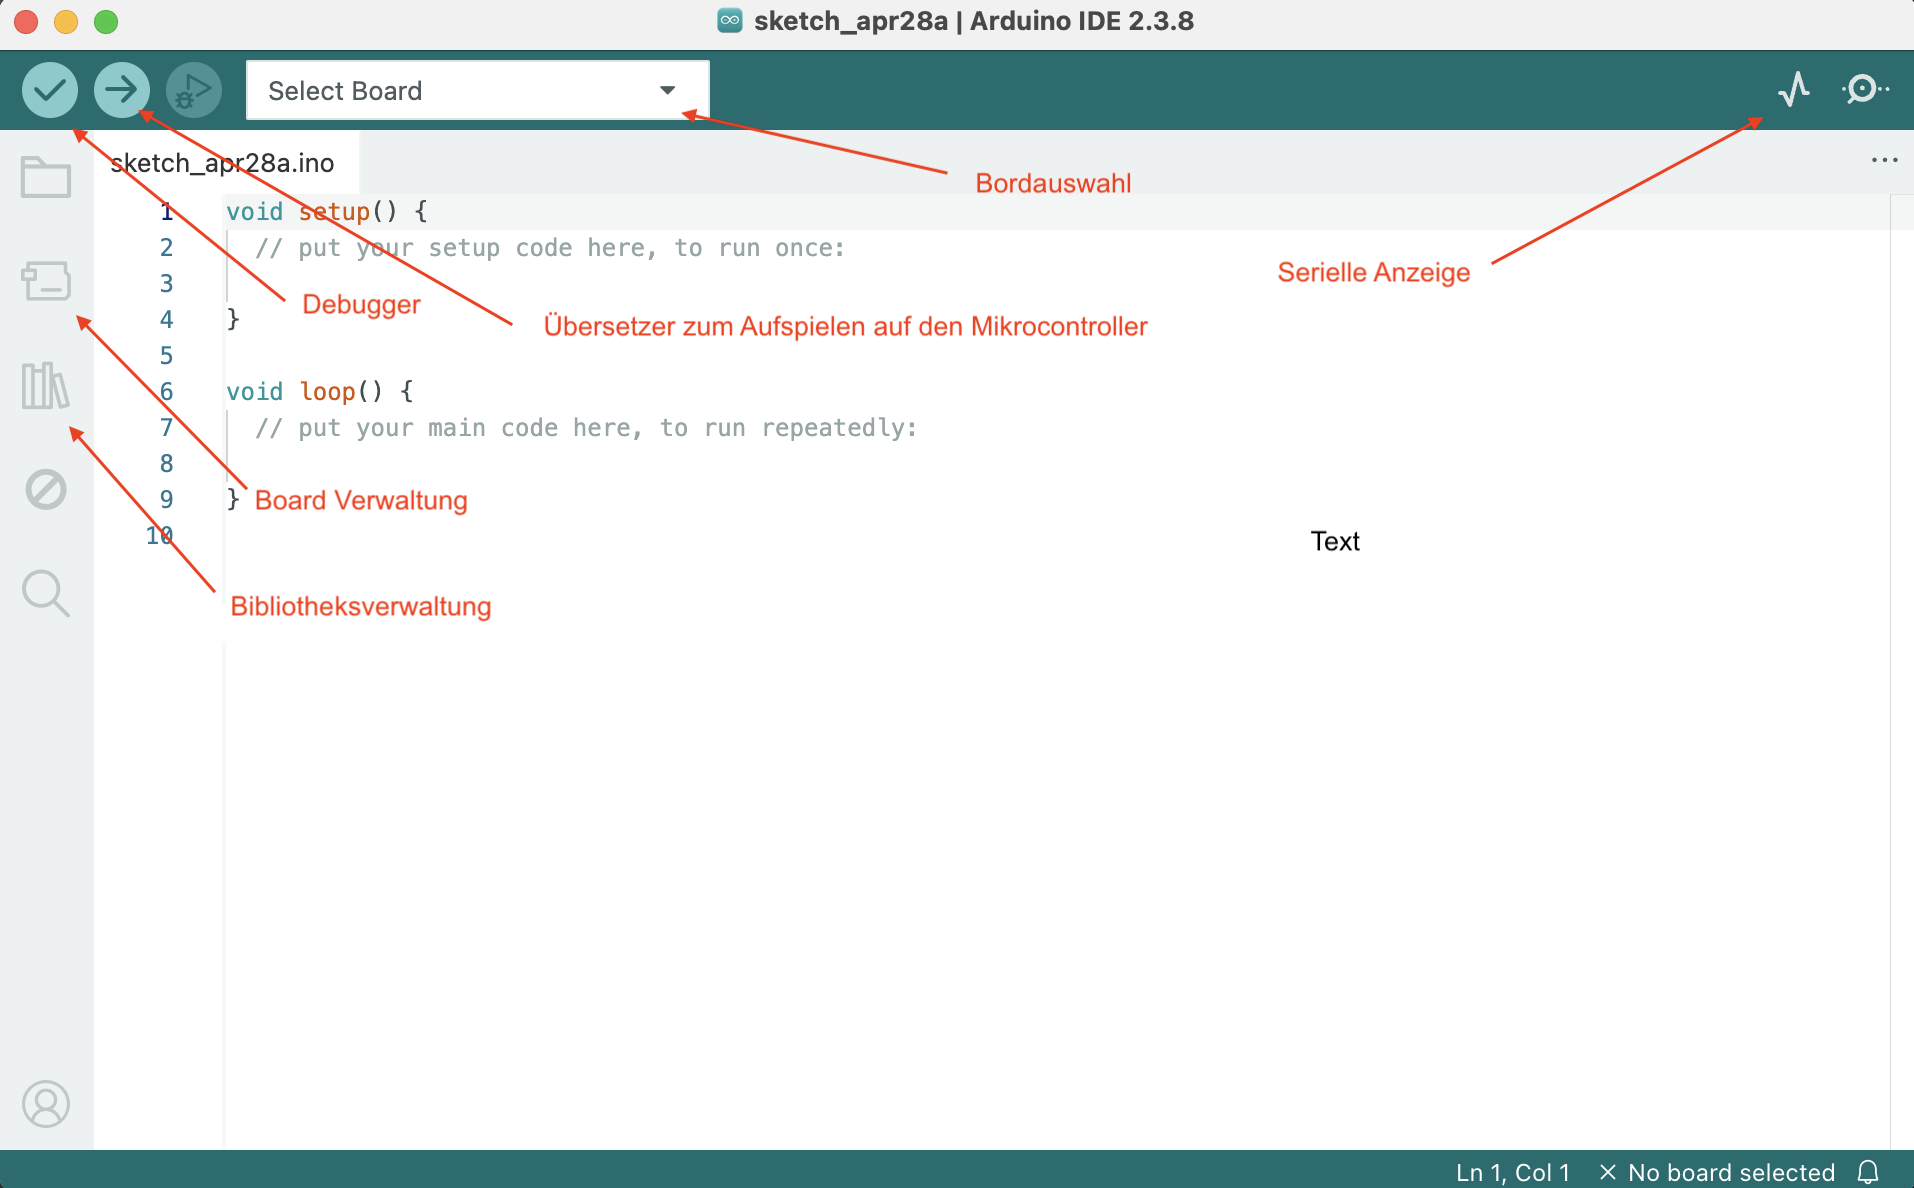
\includegraphics[width=1\textwidth,keepaspectratio]{../../Images/ArduinoIDE/MacOS/ArduinoIDEGUI}
	\caption{Übersicht der Arduino IDE und Beschriftung der einzelnen Untermenüs  }
	\label{pic:ArduinoIDEGUIMac}
\end{figure}
\end{center}
\textbf{HIER WEITER SCHREIBEN }



%\begin{center}
%	\includegraphics[width=1\textwidth,keepaspectratio]{../../Images/ArduinoIDE/MacOS/IDEMac03}
%	\captionof{figure}{Download der Arduino IDE starten}
%	\label{pic:IDEMac03}
%\end{center}
%
%Es erscheint eine Spendenanfrage. Sie können freiwillig spenden oder über \glqq JUST DOWNLOAD \grqq fortfahren (vgl. Abbildung~\ref{pic:IDEMac04}).
%
%\begin{center}
%	\includegraphics[width=1\textwidth,keepaspectratio]{../../Images/ArduinoIDE/MacOS/IDEMac04}
%	\captionof{figure}{Optional: Spendenaufruf beim Download}
%	\label{pic:IDEMac04}
%\end{center}
%
%Vor dem Download können Sie optional den Newsletter abonnieren, vgl. Abbildung~\ref{pic:IDEMac05}.
%
%\begin{center}
%	\includegraphics[width=1\textwidth,keepaspectratio]{../../Images/ArduinoIDE/MacOS/IDEMac05}
%	\captionof{figure}{Optional: Newsletter abonnieren}
%	\label{pic:IDEMac05}
%\end{center}
%
%Da es sich um ein Programm aus dem Internet handelt, muss der Download zunächst erlaubt werden, vgl. Abbildung~\ref{pic:IDEMac06}.
%
%\begin{center}
%	\includegraphics[width=1\textwidth,keepaspectratio]{../../Images/ArduinoIDE/MacOS/IDEMac06}
%	\captionof{figure}{Download-Erlaubnis erteilen}
%	\label{pic:IDEMac06}
%\end{center}
%
%Über den Pfeil oben rechts lässt sich der Fortschritt anzeigen (vgl. Abbildung~\ref{pic:IDEMac07}).
%
%\begin{center}
%	\includegraphics[width=1\textwidth,keepaspectratio]{../../Images/ArduinoIDE/MacOS/IDEMac07}
%	\captionof{figure}{Download-Fortschritt einsehen}
%	\label{pic:IDEMac07}
%\end{center}
%
%Öffnen Sie nach dem Download die Datei per Doppelklick (vgl. Abbildung~\ref{pic:IDEMac08}).
%
%\begin{center}
%	\includegraphics[width=1\textwidth,keepaspectratio]{../../Images/ArduinoIDE/MacOS/IDEMac08}
%	\captionof{figure}{Heruntergeladene Datei öffnen}
%	\label{pic:IDEMac08}
%\end{center}
%
%Ziehen Sie nun die App in den Programme-Ordner (vgl. Abbildung~\ref{pic:IDEMac10}).
%
%\begin{center}
%	\includegraphics[width=1\textwidth,keepaspectratio]{../../Images/ArduinoIDE/MacOS/IDEMac10}
%	\captionof{figure}{Installation durch Ziehen in den Programme-Ordner}
%	\label{pic:IDEMac10}
%\end{center}
%
%Die Installation ist abgeschlossen. Öffnen Sie die App über den Programme-Ordner (vgl. Abbildung~\ref{pic:IDEMac11}).
%
%\begin{center}
%	\includegraphics[width=1\textwidth,keepaspectratio]{../../Images/ArduinoIDE/MacOS/IDEMac11}
%	\captionof{figure}{Arduino IDE starten}
%	\label{pic:IDEMac11}
%\end{center}
%
%Bestätigen Sie die Sicherheitsabfrage mit \glqq Öffnen\grqq (vgl. Abbildung~\ref{pic:IDEMac12}).
%
%\begin{center}
%	\includegraphics[width=1\textwidth,keepaspectratio]{../../Images/ArduinoIDE/MacOS/IDEMac12}
%	\captionof{figure}{Sicherheitsabfrage bei erstmaligem Start}
%	\label{pic:IDEMac12}
%\end{center}
%
%\subsection{Bibliotheken installieren}
%\label{Bibliotheken installieren Mac}
%
%Klicken Sie auf das Buch-Symbol (vgl. Abbildung~\ref{pic:IDEMac13}) und suchen Sie die gewünschte Bibliothek. Die vollständige Liste finden Sie in Kapitel \ref{Bibliotheken}. Installieren Sie jede Bibliothek durch Klick auf \glqq Install \grqq.
%
%\begin{center}
%	\includegraphics[width=1\textwidth,keepaspectratio]{../../Images/ArduinoIDE/MacOS/IDEMac13}
%	\captionof{figure}{Bibliotheken-Suchmaske der Arduino IDE}
%	\label{pic:IDEMac13}
%\end{center}
%
%Abbildung~\ref{pic:IDEMac14} zeigt eine erfolgreich installierte Bibliothek.
%
%\begin{center}
%	\includegraphics[width=1\textwidth,keepaspectratio]{../../Images/ArduinoIDE/MacOS/IDEMac14}
%	\captionof{figure}{Erfolgreiche Installation einer Bibliothek}
%	\label{pic:IDEMac14}
%\end{center}
%
%\subsection{Board Manager}
%
%Mit dem Board Manager können Sie zusätzliche Boards hinzufügen (vgl. Abbildung~\ref{pic:IDEMac15}). Suchen Sie zum Beispiel nach dem \glqq ESP \grqq oder \glqq Nano 33 BLE Sense \grqq und installieren Sie das passende Board. 
%\begin{center}
%	\includegraphics[width=1\textwidth,keepaspectratio]{../../Images/ArduinoIDE/MacOS/IDEMac15}
%	\captionof{figure}{Der Board Manager in der Arduino IDE}
%	\label{pic:IDEMac15}
%\end{center}
%
%\label{PortauswahlMAC}
%Klappen Sie das USB-Menü aus (vgl. Abbildung~\ref{pic:IDEMac16}) und wählen Sie \glqq Select other board and port\grqq.
%
%\begin{center}
%	\includegraphics[width=1\textwidth,keepaspectratio]{../../Images/ArduinoIDE/MacOS/IDEMac16}
%	\captionof{figure}{Board- und Portauswahl öffnen}
%	\label{pic:IDEMac16}
%\end{center}
%
%Geben Sie \glqq Nano 33 BLE Sense\grqq in das Suchfeld ein, verbinden Sie das Board und wählen Sie den richtigen Port (vgl. Abbildung~\ref{pic:IDEMac17}).
%
%\begin{center}
%	\includegraphics[width=1\textwidth,keepaspectratio]{../../Images/ArduinoIDE/MacOS/IDEMac17}
%	\captionof{figure}{Passenden Board und Port auswählen}
%	\label{pic:IDEMac17}
%\end{center}
%
%\subsection{Beispielprogramm \glqq Blink\grqq}
%
%Wählen Sie den Pfad gemäß Abbildung~\ref{pic:IDEMac18}, um ein Beispielprogramm zu laden.
%
%\begin{center}
%	\includegraphics[width=1\textwidth,keepaspectratio]{../../Images/ArduinoIDE/MacOS/IDEMac18}
%	\captionof{figure}{Beispielprogramme öffnen}
%	\label{pic:IDEMac18}
%\end{center}
%
%Das Blink-Programm wird geöffnet (vgl. Abbildung~\ref{pic:IDEMac19}) und kann nach Auswahl des Ports hochgeladen werden (siehe \ref{PortauswahlMAC}). Die Kompilierung erfolgt automatisch vor dem Upload oder manuell über das Häkchen-Symbol.
%
%\begin{center}
%	\includegraphics[width=1\textwidth,keepaspectratio]{../../Images/ArduinoIDE/MacOS/IDEMac19}
%	\captionof{figure}{Das geöffnete Beispielprogramm \glqq Blink\grqq}
%	\label{pic:IDEMac19}
%\end{center}
%
%Nach erfolgreichem Upload erscheint ein Terminalfenster mit einer Bestätigung.
%


